\documentclass[12pt, a4paper]{report}
\usepackage[utf8]{inputenc}
\usepackage[spanish]{babel}
\usepackage{float}
\usepackage{geometry} % márgenes
\usepackage[conEntregas]{caratula} % carátula

\begin{document}

% **************************************************************************
%
%  Package 'caratula', version 0.5 (para componer caratulas de TPs del DC).
%
%  En caso de dudas, problemas o sugerencias sobre este package escribir a
%  Brian J. Cardiff (bcardif arroba gmail.com).
%  Nico Rosner (nrosner arroba dc.uba.ar).
%
% **************************************************************************

% ----- Informacion sobre el package para el sistema -----------------------

\NeedsTeXFormat{LaTeX2e}
\ProvidesPackage{caratula}[2013/08/04 v0.5 Para componer caratulas de TPs del DC]
\RequirePackage{ifthen}
\usepackage[pdftex]{graphicx}

% ----- Imprimir un mensajito al procesar un .tex que use este package -----

\typeout{Cargando package 'caratula' v0.5 (2013/08/04)}

% ----- Algunas variables --------------------------------------------------

\let\Materia\relax
\let\Submateria\relax
\let\Titulo\relax
\let\Subtitulo\relax
\let\Grupo\relax
\let\Fecha\relax
\let\Logoimagefile\relax
\newcommand{\LabelIntegrantes}{}
\newboolean{showLU}
\newboolean{showEntregas}
\newboolean{showDirectores}
\newboolean{showCoDirectores}

% ----- Comandos para que el usuario defina las variables ------------------

\def\materia#1{\def\Materia{#1}}
\def\submateria#1{\def\Submateria{#1}}
\def\titulo#1{\def\Titulo{#1}}
\def\subtitulo#1{\def\Subtitulo{#1}}
\def\grupo#1{\def\Grupo{#1}}
\def\fecha#1{\def\Fecha{#1}}
\def\logoimagefile#1{\def\Logoimagefile{#1}}

% ----- Token list para los integrantes ------------------------------------

\newtoks\intlist\intlist={}

\newtoks\intlistSinLU\intlistSinLU={}

\newcounter{integrantesCount}
\setcounter{integrantesCount}{0}
\newtoks\intTabNombre\intTabNombre={}
\newtoks\intTabLU\intTabLU={}
\newtoks\intTabEmail\intTabEmail={}

\newcounter{directoresCount}
\setcounter{directoresCount}{0}
\newtoks\direcTabNombre\direcTabNombre={}
\newtoks\direcTabEmail\direcTabEmail={}

\newcounter{coDirectoresCount}
\setcounter{coDirectoresCount}{0}
\newtoks\codirecTabNombre\codirecTabNombre={}
\newtoks\codirecTabEmail\codirecTabEmail={}


% ----- Comando para que el usuario agregue integrantes --------------------

\def\integrante#1#2#3{%
    \intlist=\expandafter{\the\intlist\rule{0pt}{1.2em}#1&#2&\tt #3\\[0.2em]}%
    \intlistSinLU=\expandafter{\the\intlistSinLU\rule{0pt}{1.2em}#1 & \tt #3\\[0.2em]}%
    %
    \ifthenelse{\value{integrantesCount} > 0}{%
        \intTabNombre=\expandafter{\the\intTabNombre & #1}%
        \intTabLU=\expandafter{\the\intTabLU & #2}%
        \intTabEmail=\expandafter{\the\intTabEmail & \tt #3}%
    }{
        \intTabNombre=\expandafter{\the\intTabNombre #1}%
        \intTabLU=\expandafter{\the\intTabLU #2}%
        \intTabEmail=\expandafter{\the\intTabEmail \tt #3}%
    }%
    \addtocounter{integrantesCount}{1}%
}

\def\director#1#2{%
    \ifthenelse{\value{directoresCount} > 0}{%
        \direcTabNombre=\expandafter{\the\direcTabNombre & #1}%
        \direcTabEmail=\expandafter{\the\direcTabEmail & \tt #2}%
    }{
        \direcTabNombre=\expandafter{\the\direcTabNombre #1}%
        \direcTabEmail=\expandafter{\the\direcTabEmail \tt #2}%
    }%
    \addtocounter{directoresCount}{1}%
}

\def\codirector#1#2{%
    \ifthenelse{\value{coDirectoresCount} > 0}{%
        \codirecTabNombre=\expandafter{\the\codirecTabNombre & #1}%
        \codirecTabEmail=\expandafter{\the\codirecTabEmail & \tt #2}%
    }{
        \codirecTabNombre=\expandafter{\the\codirecTabNombre #1}%
        \codirecTabEmail=\expandafter{\the\codirecTabEmail \tt #2}%
    }%
    \addtocounter{coDirectoresCount}{1}%
}


% ----- Macro para generar la tabla de integrantes -------------------------

\newcommand{\tablaIntegrantes}{\ }

\newcommand{\tablaIntegrantesVertical}{%
\ifthenelse{\boolean{showLU}}{%
    \begin{tabular}[t]{| l @{\hspace{4ex}} c @{\hspace{4ex}} l|}
        \hline
        \multicolumn{1}{|c}{\rule{0pt}{1.2em} \LabelIntegrantes} & LU &  \multicolumn{1}{c|}{Correo electr\'onico} \\[0.2em]
        \hline \hline
        \the\intlist
        \hline
    \end{tabular}
}{
    \begin{tabular}[t]{| l @{\hspace{4ex}} @{\hspace{4ex}} l|}
        \hline
        \multicolumn{1}{|c}{\rule{0pt}{1.2em} \LabelIntegrantes} &  \multicolumn{1}{c|}{Correo electr\'onico} \\[0.2em]
        \hline \hline
        \the\intlistSinLU
        \hline
    \end{tabular}
    }%
}

\newcommand{\tablaIntegrantesHorizontal}{%
    \begin{tabular}[t]{ *{\value{integrantesCount}}{c} }
    \the\intTabNombre \\%
\ifthenelse{\boolean{showLU}}{
    \the\intTabLU \\%
}{}
    \the\intTabEmail %
    \end{tabular}%
}

\newcommand{\tablaDirectores}{%
\ifthenelse{\boolean{showDirectores}}{%
	\bigskip
	Directores

	\smallskip
    \begin{tabular}[t]{ *{\value{directoresCount}}{c} }
    \the\direcTabNombre \\%
    \the\direcTabEmail %
    \end{tabular}%
}{}%
}

\newcommand{\tablaCoDirectores}{%
\ifthenelse{\boolean{showCoDirectores}}{%
	\bigskip
	Co-Directores

	\smallskip
    \begin{tabular}[t]{ *{\value{coDirectoresCount}}{c} }
    \the\codirecTabNombre \\%
    \the\codirecTabEmail %
    \end{tabular}%
}{}%
}

\newcommand{\tablaEntregas}{%
\ifthenelse{\boolean{showEntregas}}{%
  \bigskip%
  \begin{tabular}[t]{|l p{3.5cm} p{1.5cm}|}%
  \hline%
  \rule{0pt}{1.2em} Instancia & Docente & Nota \\[0.2em] %
  \hline%
  \hline%
  \rule{0pt}{1.2em} Primera entrega & & \\[0.2em] %
  \hline%
  \rule{0pt}{1.2em} Segunda entrega & & \\[0.2em] %
  \hline%
  \end{tabular}%
}{}%
}

% ----- Codigo para manejo de errores --------------------------------------

\def\se{\let\ifsetuperror\iftrue}
\def\ifsetuperror{%
    \let\ifsetuperror\iffalse
    \ifx\Materia\relax\se\errhelp={Te olvidaste de proveer una \materia{}.}\fi
    \ifx\Titulo\relax\se\errhelp={Te olvidaste de proveer un \titulo{}.}\fi
    \edef\mlist{\the\intlist}\ifx\mlist\empty\se%
    \errhelp={Tenes que proveer al menos un \integrante{nombre}{lu}{email}.}\fi
    \expandafter\ifsetuperror}

\def\aftermaketitle{%
  \setcounter{page}{1}
}

% ----- \maketitletxt correspondiente a la versi�n v0.2.1 (texto v0.2 + fecha ) ---------

\def\maketitletxt{%
    \ifsetuperror\errmessage{Faltan datos de la caratula! Ingresar 'h' para mas informacion.}\fi
    \thispagestyle{empty}
    \begin{center}
    \vspace*{\stretch{2}}
    {\LARGE\textbf{\Materia}}\\[1em]
    \ifx\Submateria\relax\else{\Large \Submateria}\\[0.5em]\fi
    \ifx\Fecha\relax\else{\Large \Fecha}\\[0.5em]\fi
    \par\vspace{\stretch{1}}
    {\large Departamento de Computaci\'on}\\[0.5em]
    {\large Facultad de Ciencias Exactas y Naturales}\\[0.5em]
    {\large Universidad de Buenos Aires}
    \par\vspace{\stretch{3}}
    {\Large \textbf{\Titulo}}\\[0.8em]
    {\Large \Subtitulo}
    \par\vspace{\stretch{3}}
    \ifx\Grupo\relax\else\textbf{\Grupo}\par\bigskip\fi
    \tablaIntegrantes
    \end{center}
    \vspace*{\stretch{3}}
    \newpage\aftermaketitle}

% ----- \maketitletxtlogo correspondiente v0.2.1 (texto con fecha y logo) ---------

\def\maketitletxtlogo{%
    \ifsetuperror\errmessage{Faltan datos de la caratula! Ingresar 'h' para mas informacion.}\fi
    \thispagestyle{empty}
    \begin{center}
    \ifx\Logoimagefile\relax\else\includegraphics{\Logoimagefile}\fi \hfill 
\includegraphics{logo_dc.jpg}\\[1em]
    \vspace*{\stretch{2}}
    {\LARGE\textbf{\Materia}}\\[1em]
    \ifx\Submateria\relax\else{\Large \Submateria}\\[0.5em]\fi
    \ifx\Fecha\relax\else{\large \Fecha}\\[0.5em]\fi
    \par\vspace{\stretch{1}}
    {\large Departamento de Computaci\'on}\\[0.5em]
    {\large Facultad de Ciencias Exactas y Naturales}\\[0.5em]
    {\large Universidad de Buenos Aires}
    \par\vspace{\stretch{3}}
    {\Large \textbf{\Titulo}}\\[0.8em]
    {\Large \Subtitulo}
    \par\vspace{\stretch{3}}
    \ifx\Grupo\relax\else\textbf{\Grupo}\par\bigskip\fi
    \tablaIntegrantes
    \end{center}
    \vspace*{\stretch{4}}
    \newpage\aftermaketitle}

% ----- \maketitlegraf correspondiente a la versi�n v0.3 (gr�fica) -------------

\def\maketitlegraf{%
    \ifsetuperror\errmessage{Faltan datos de la caratula! Ingresar 'h' para mas informacion.}\fi
%
    \thispagestyle{empty}

    \ifx\Logoimagefile\relax\else\includegraphics{\Logoimagefile}\fi \hfill 
\includegraphics{logo_dc.jpg}

    \vspace*{.06 \textheight}

    \noindent \textbf{\huge \Titulo}  \medskip \\
    \ifx\Subtitulo\relax\else\noindent\textbf{\large \Subtitulo} \\ \fi%
    \noindent \rule{\textwidth}{1 pt}

    {\noindent\large\Fecha \hspace*\fill \Materia} \\
    \ifx\Submateria\relax\else{\noindent \hspace*\fill \Submateria}\fi%

    \medskip%
    \begin{center}
        \ifx\Grupo\relax\else\textbf{\Grupo}\par\bigskip\fi
        \tablaIntegrantes

        \tablaDirectores

        \tablaCoDirectores

      %  \tablaEntregas
    \end{center}%
    \vfill%
%
    \begin{minipage}[t]{\textwidth}
        \begin{minipage}[t]{.55 \textwidth}
            
\includegraphics{logo_uba.jpg}
        \end{minipage}%%
        \begin{minipage}[b]{.45 \textwidth}
            \textbf{\textsf{Facultad de Ciencias Exactas y Naturales}} \\
            \textsf{Universidad de Buenos Aires} \\
            {\scriptsize %
            Ciudad Universitaria - (Pabell\'on I/Planta Baja) \\
                Intendente G\"uiraldes 2610 - C1428EGA \\
            Ciudad Aut\'onoma de Buenos Aires - Rep. Argentina \\
                Tel/Fax: (++54 +11) 4576-3300 \\
            http://www.exactas.uba.ar \\
            }
        \end{minipage}
    \end{minipage}%
%
    \newpage\aftermaketitle}

% ----- Reemplazamos el comando \maketitle de LaTeX con el nuestro ---------
\renewcommand{\maketitle}{\maketitlegraf}

% ----- Dependiendo de las opciones ---------
%
% opciones:
%   txt     : caratula solo texto.
%   txtlogo : caratula txt con logo del DC y del grupo (opcional).
%   graf    : (default) caratula grafica con logo del DC, UBA y del grupo (opcional).
%
\@makeother\*% some package redefined it as a letter (as color.sty)
%
% Layout general de la caratula
%
\DeclareOption{txt}{\renewcommand{\maketitle}{\maketitletxt}}
\DeclareOption{txtlogo}{\renewcommand{\maketitle}{\maketitletxtlogo}}
\DeclareOption{graf}{\renewcommand{\maketitle}{\maketitlegraf}}
%
% Etiqueta Autores o Integrantes
%
\DeclareOption{integrante}{\renewcommand{\LabelIntegrantes}{Integrante}}
\DeclareOption{autor}{\renewcommand{\LabelIntegrantes}{Autor}}
%
% Formato tabla de integrantes
%
\DeclareOption{intVert}{\renewcommand{\tablaIntegrantes}{\tablaIntegrantesVertical}}
\DeclareOption{intHoriz}{\renewcommand{\tablaIntegrantes}{\tablaIntegrantesHorizontal}}
\DeclareOption{conLU}{\setboolean{showLU}{true}}
\DeclareOption{sinLU}{\setboolean{showLU}{false}}
\DeclareOption{conEntregas}{\setboolean{showEntregas}{true}}
\DeclareOption{sinEntregas}{\setboolean{showEntregas}{false}}
\DeclareOption{showDirectores}{\setboolean{showDirectores}{true}}
\DeclareOption{hideDirectores}{\setboolean{showDirectores}{false}}
\DeclareOption{showCoDirectores}{\setboolean{showCoDirectores}{true}}
\DeclareOption{hideCoDirectores}{\setboolean{showCoDirectores}{false}}
%
% Opciones predeterminadas
%
\ExecuteOptions{intVert}%
\ExecuteOptions{graf}%
\ExecuteOptions{integrante}%
\ExecuteOptions{conLU}%
\ExecuteOptions{hideDirectores}%
\ExecuteOptions{hideCoDirectores}%
\ExecuteOptions{sinEntregas}%
%
\ProcessOptions\relax


\tableofcontents{}
\begin{abstract}
    El objetivo de este trabajo práctico es ver como se puede utilizar
la regresión polinomial para estimar un conjunto de datos mediante
polinomios. \par
\indent Para tener una forma de medir y comparar los resultados, 
se presentán funciones de error y se analiza como 
afecta al vector que los minimiza. \par 
\indent Luego se presentará una conocida
set datos ("Boston Housing Dataset") y la forma de calcular la matriz de
correlación, junto con un breve analizasis de la feature MEDV
del set datos.
\end{abstract}

\chapter{Introducción teórica} 


\section{Regresión polinomial}
Queremos predecir valores de la primera en función de valores observados
de la segunda.El análisis de regresión consiste en ajustar un modelo
a los datos, estimando coeficientes a partir de las observaciones, con 
el fin de predecir valores de la variable de respuesta a partir de una 
(regresión simple) o más variables (regresión multiple) predictivas o 
explicativas.\par
\indent El análisis de regresión se puede usar para:
\begin{itemize}
    \item identificar a las variables predictivas relacionadas con una variable de respuesta
    \item describir la forma de la relación entre estas variables y para derivar una función matemática óptima que modele esta relación
    \item predecir la variable de respuesta a partir de la(s) explicativas o predictoras
\end{itemize}
\subsection{Definiciones}
\begin{itemize}
    \item $M =$ grado del polinomio interpolante.
    \item $N =$ cantidad de datos.
    \item $X_{i} = (x_{i}^{0},...,x_{i}^{M}).$
    \item $ W = (w_{0},...,w_{M}).$
    \item $ Y(X,W) = XW^{T}.$
    \item $E_{D}(W) = (1/2)  \sum_{i=1}^{N} (Y(X_{i},W)-t_{i})^{2}$
    \item $E(W) = (1/2)  \sum_{i=1}^{N} (Y(X_{i},W)-t_{i})^{2} + (\lambda/2)||W||_{2}$
    \item $E_{RMS}(W) = \sqrt{2E(W)/N}$.
    \item $E_{DRMS}(W) = \sqrt{2E_{D}(W)/N}$.
\end{itemize}

Dado que la función $E(W)$ es convexa en w, está posee un
minimo y esté es único.\par
\subsection{Objetivo}
\indent Buscar cual es el W que minimice los errores de
$Y(X_{i},W)-t_{i}$.
\section{Boston Housing Dataset}
The dataset contains a total of 506 cases.\par
\indent Hay 14 atributos en cada caso del conjunto de datos.
\begin{itemize}
    \item CRIM - tasa de criminalidad per cápita por ciudad
    \item ZN - proporción de tierra residencial dividida en zonas para lotes de más de 25,000 pies cuadrados.
    \item INDUS - proporción de acres de negocios no comerciales por ciudad.
    \item CHAS - Variable ficticia del río Charles (1 si el tramo limita con el río; 0 si no)
    \item NOX - concentración de óxidos nítricos (partes por 10 millones)
    \item RM - número medio de habitaciones por vivienda
    \item AGE - proporción de unidades ocupadas por sus propietarios construidas antes de 1940
    \item DIS - distancias ponderadas a cinco centros de empleo de Boston
    \item RAD - índice de accesibilidad a carreteras radiales
    \item TAX - tasa del impuesto sobre el valor total de la propiedad por cada 10,000
    \item PTRATIO - número de alumnos por docente y por ciudad
    \item B - 1000(Bk - 0.63)$^{2}$ donde Bk es la proporción de negros por ciudad
    \item LSTAT - menor condición de la población
    \item MEDV - Valor medio de las viviendas ocupadas por sus propietarios en miles de dólares.
\end{itemize}

\chapter{Desarrollo}
El desarrollado de este trabajo pretende hacer un análisis de como afecta
la concideración de diferentes funciones de error al vector solución y la 
variación de la media y varianza muestrales de los errores.

\section{Regresión Polinomial}
Se implementan funciones de error.\par
\indent Se realiza un analisis de el valor medio y la desviación 
standard muestrales para cada grado de polinomio considerado.\par
\indent Graficamos la influencia del grado del polinomio
sobre el $E_{RMS}$
\section{Boston Housing Dataset}
Lo que se busca es mostrar las relaciones entre
las features de este set de datos.\par
\indent Para ellos graficaremos los scatter-plot de todos
los features y la matriz de correlación.\par
\indent Luego para aquellas features que presenten
un coeficiente de correlación con la feature MEDV mayor
a 0.5 en valor absoluto se ajustan con polinomios de grado
1, 2 y 3, se grafican los scatter-plot correspondientes
y se calculan los $E_{RMS}$.


\chapter{Experimentación}
\section{variación de los grados de Polinomios}


\begin{figure}[h]
    \centering
    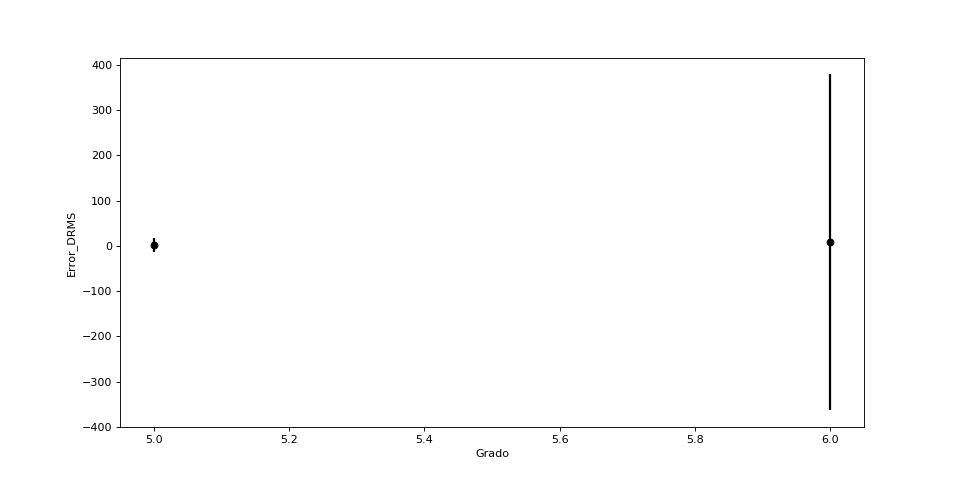
\includegraphics[width=\textwidth]{1_6.png}
    \caption{}
    \label{}
\end{figure}
\begin{figure}[h]
    \centering
    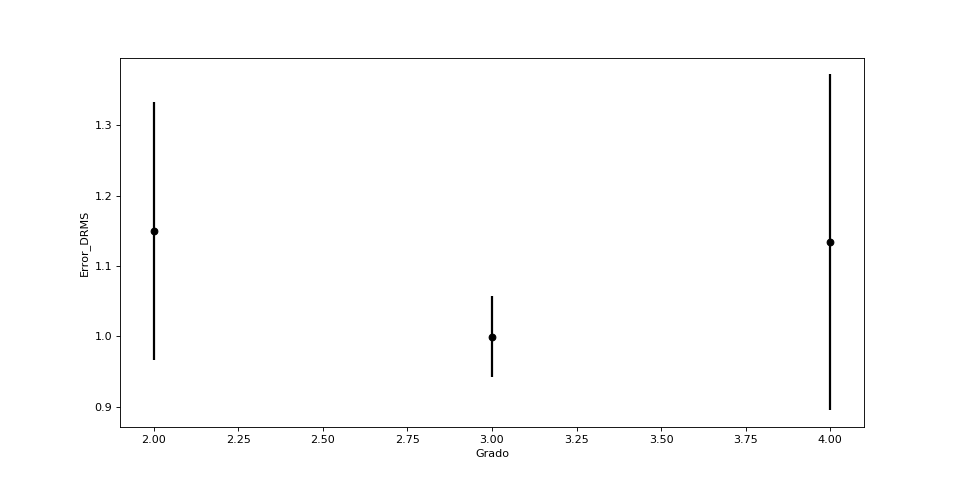
\includegraphics[width=\textwidth]{2_4.png}
    \caption{}
    \label{}
\end{figure}
\begin{figure}[h]
    \centering
    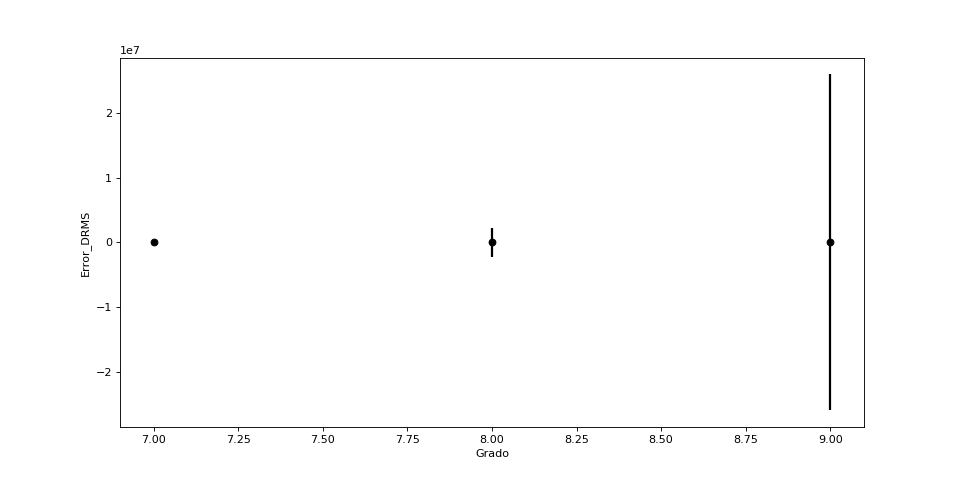
\includegraphics[width=\textwidth]{2_9.png}
    \caption{}
    \label{}
\end{figure}

\begin{figure}[h]
    \centering
    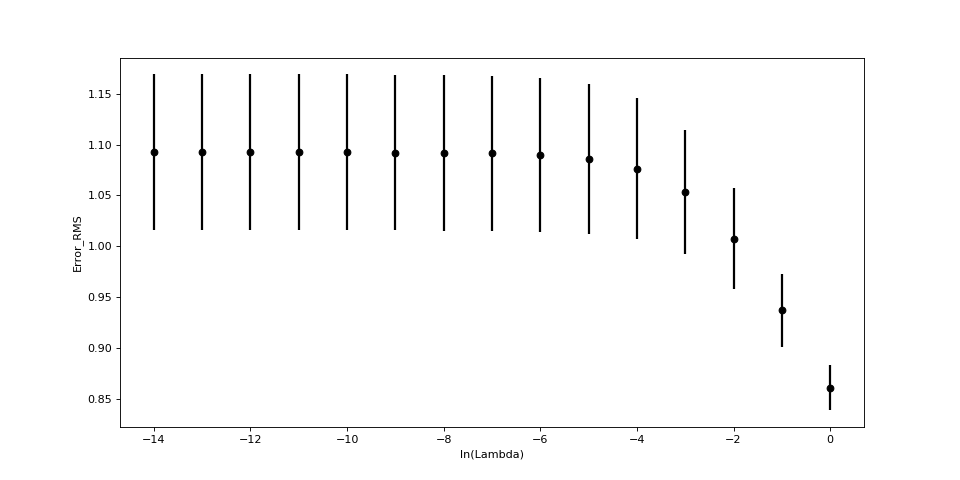
\includegraphics[width=\textwidth]{error_INDUS_lambda.png}
    \caption{}
    \label{error_INDUS_lambda}
\end{figure}
\begin{figure}[h]
    \centering
    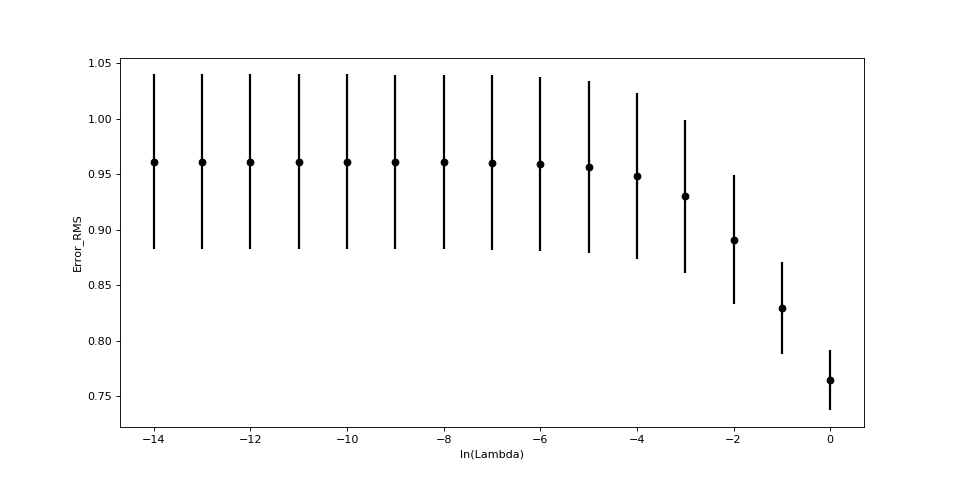
\includegraphics[width=\textwidth]{error_INDUSNOXRMAGETAX_lambda.png}
    \caption{}
    \label{error_INDUSNOXRMAGETAX_lambda}
\end{figure}
\begin{figure}[h]
    \centering
    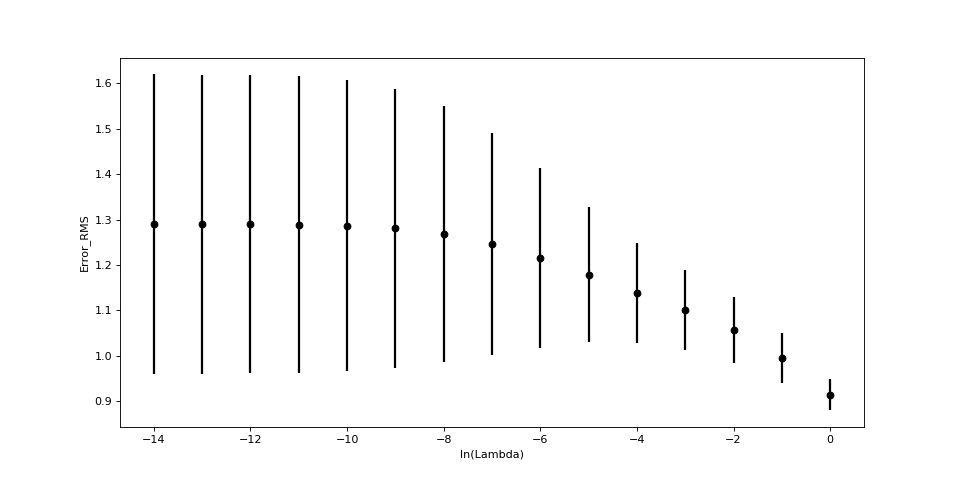
\includegraphics[width=\textwidth]{error_NOX_lambda.png}
    \caption{}
    \label{error_NOX_lambda}
\end{figure}




\begin{figure}[h]
    \centering
    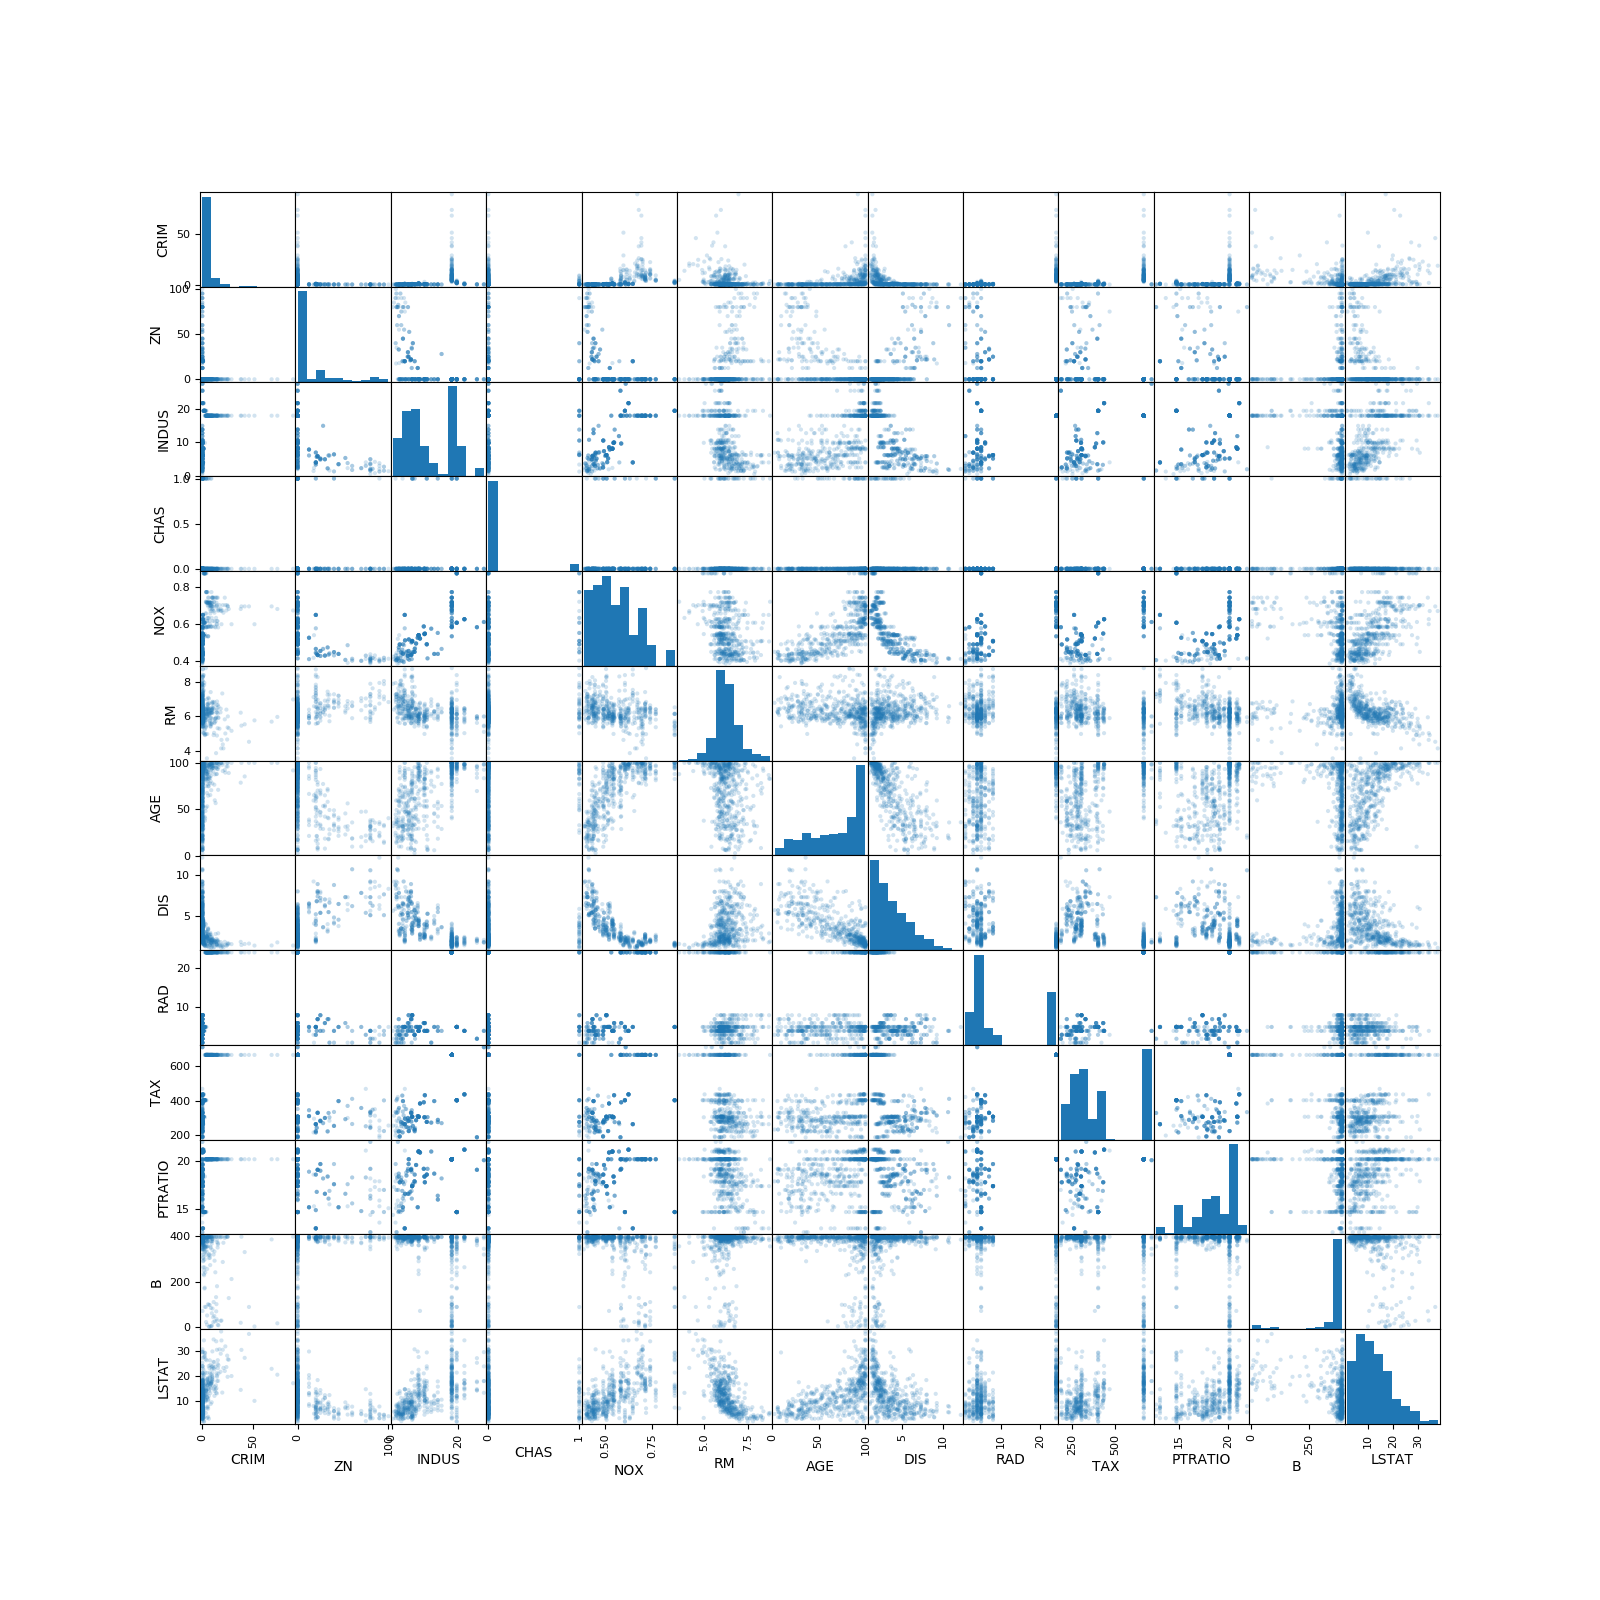
\includegraphics[width=\textwidth]{scatter.png}
    \caption{Scatter-plots de Boston Housing Dataset}
    \label{scatter}
\end{figure}
\begin{figure}[h]
    \centering
    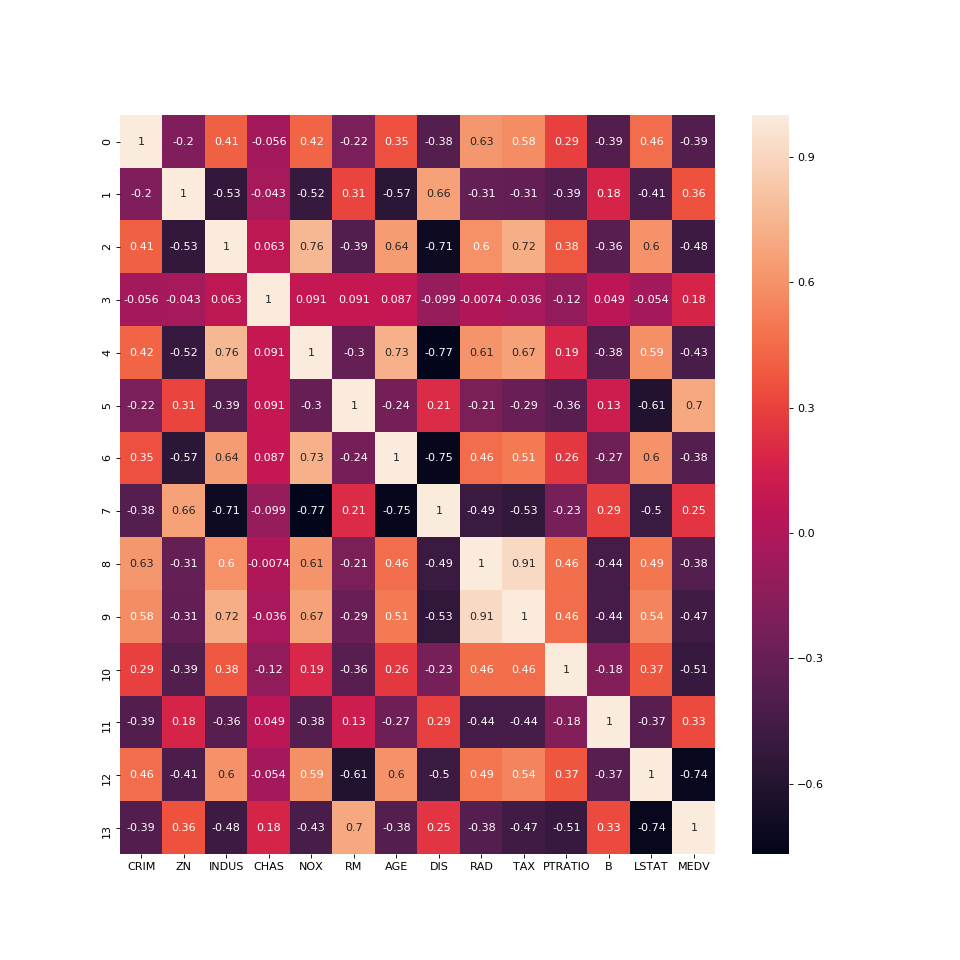
\includegraphics[width=\textwidth]{matriz_correlacion.png}
    \caption{Matriz de correlación de Boston Housing Dataset}
    \label{matriz_correlacion}
\end{figure}
\begin{figure}[h]
    \centering
    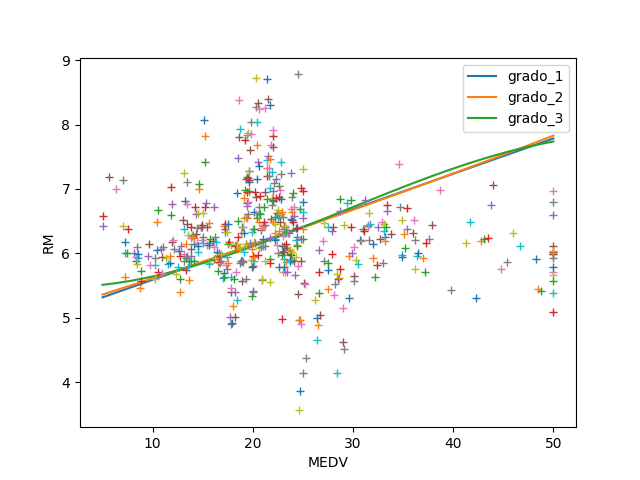
\includegraphics[width=\textwidth]{rmXmedv.png}
    \caption{Estimación de la distribución de puntos entre MEDV y RM}
    \label{rmXmedv}
\end{figure}
\begin{figure}[h]
    \centering
    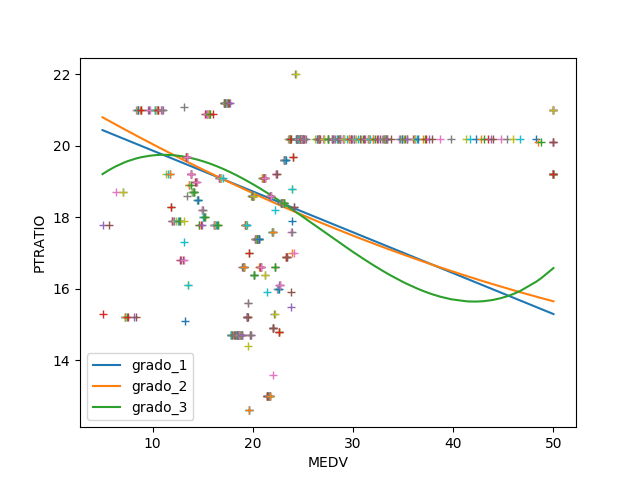
\includegraphics[width=\textwidth]{ptratioXmedv.png}
    \caption{Estimación de la distribución de puntos entre MEDV y PTRATIO}
    \label{ptratioXmedv}
\end{figure}
\begin{figure}[h]
    \centering
    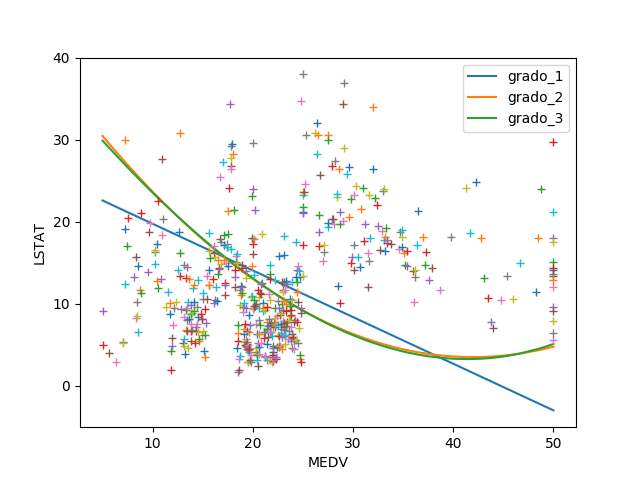
\includegraphics[width=\textwidth]{lstatXmedv.png}
    \caption{Estimación de la distribución de puntos entre MEDV y LSTAT}
    \label{lstatXmedv}
\end{figure}
\begin{figure}[h]
    \centering
    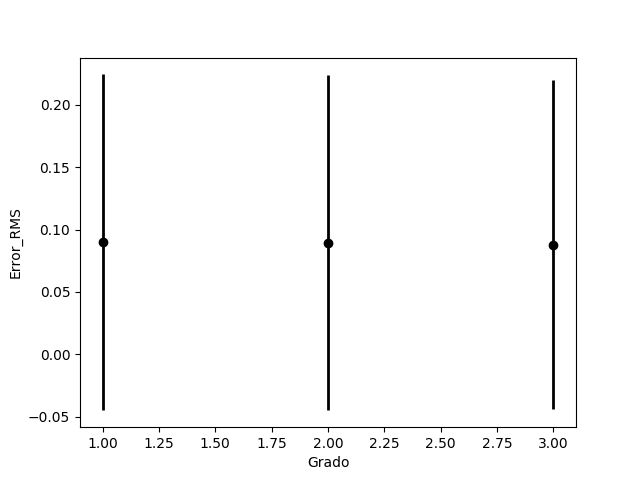
\includegraphics[width=\textwidth]{errorRM.png}
    \caption{Media y Varianza al estimar la relación entre MEDV y RM}
    \label{errorRM}
\end{figure}
\begin{figure}[h]
    \centering
    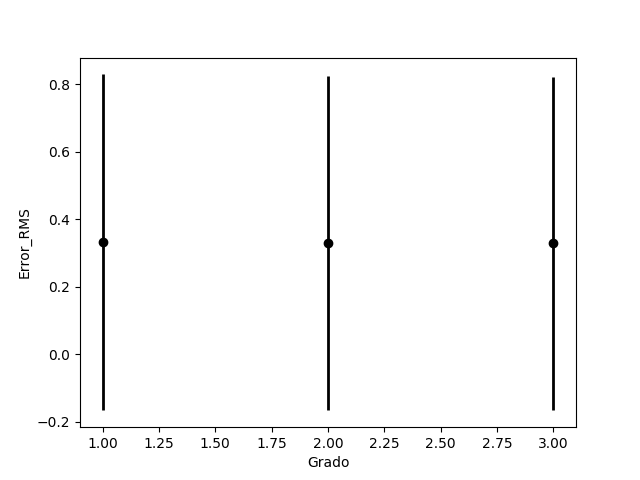
\includegraphics[width=\textwidth]{errorPTRATIO.png}
    \caption{Media y Varianza al estimar la relación entre MEDV y PTRATIO}
    \label{errorPTRATIO}
\end{figure}
\begin{figure}[h]
    \centering
    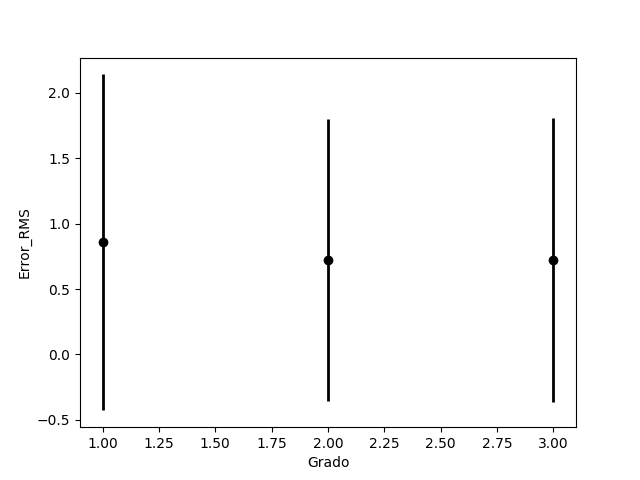
\includegraphics[width=\textwidth]{errorLSTAT.png}
    \caption{Media y Varianza al estimar la relación entre MEDV y LSTAT}
    \label{errorLSTAT}
\end{figure}

\chapter{Conclusiones}
Luego de realizar todos los experimentos y haber entendido bien el funcionamiento, podemos realizar algunas conclusiones.

\section{Referencias}
1. Pattern Recognition and Machine Learning by C. Bishop, Springer 2006. 

\end{document} 